\documentclass[12pt,a4paper]{article}
\usepackage[utf8]{inputenc}
\usepackage[portuguese]{babel}
\usepackage{geometry}
\usepackage{titlesec}
\usepackage{enumitem}
\usepackage{xcolor}
\usepackage{graphicx}
\usepackage{float}

\geometry{margin=2.5cm}
\titleformat{\section}{\Large\bfseries}{\thesection}{1em}{}
\titleformat{\subsection}{\large\bfseries}{\thesubsection}{1em}{}

\title{\textbf{Projeto de Interface com o Usuário}\\
\large Sistema de Gestão de Feiras (SGF)}
\author{Higor Roger de Freitas Santos \quad 221006440\\
Victor Eneias Oliveira \quad 221038364\\
\\
Engenharia de Software CIC0105 Turma 01 2025.1}
\date{\today}

\begin{document}

\maketitle
\tableofcontents
\newpage

\section{Fluxos de Navegação}

\subsection{Fluxo Principal de Usuário}

O sistema implementa um fluxo intuitivo que permite tanto acesso público quanto gestão autenticada:

\textbf{Fluxo para Visitantes:}
\begin{enumerate}
    \item Acesso à tela inicial
    \item Visualização de feiras disponíveis
    \item Acesso aos detalhes das feiras
    \item Opção de login para gestão
\end{enumerate}

\textbf{Fluxo para Usuários Autenticados:}
\begin{enumerate}
    \item Login/Registro via modal
    \item Acesso ao dashboard personalizado
    \item Criação e gestão de feiras
    \item Gestão de expositores e produtos
    \item Emissão de ingressos
\end{enumerate}

\subsection{Diagrama de Estados e Transições}

O diagrama a seguir apresenta os diferentes estados que um usuário pode assumir no sistema e as transições possíveis entre eles, representando o fluxo completo de navegação e interação.

\begin{figure}[H]
\centering
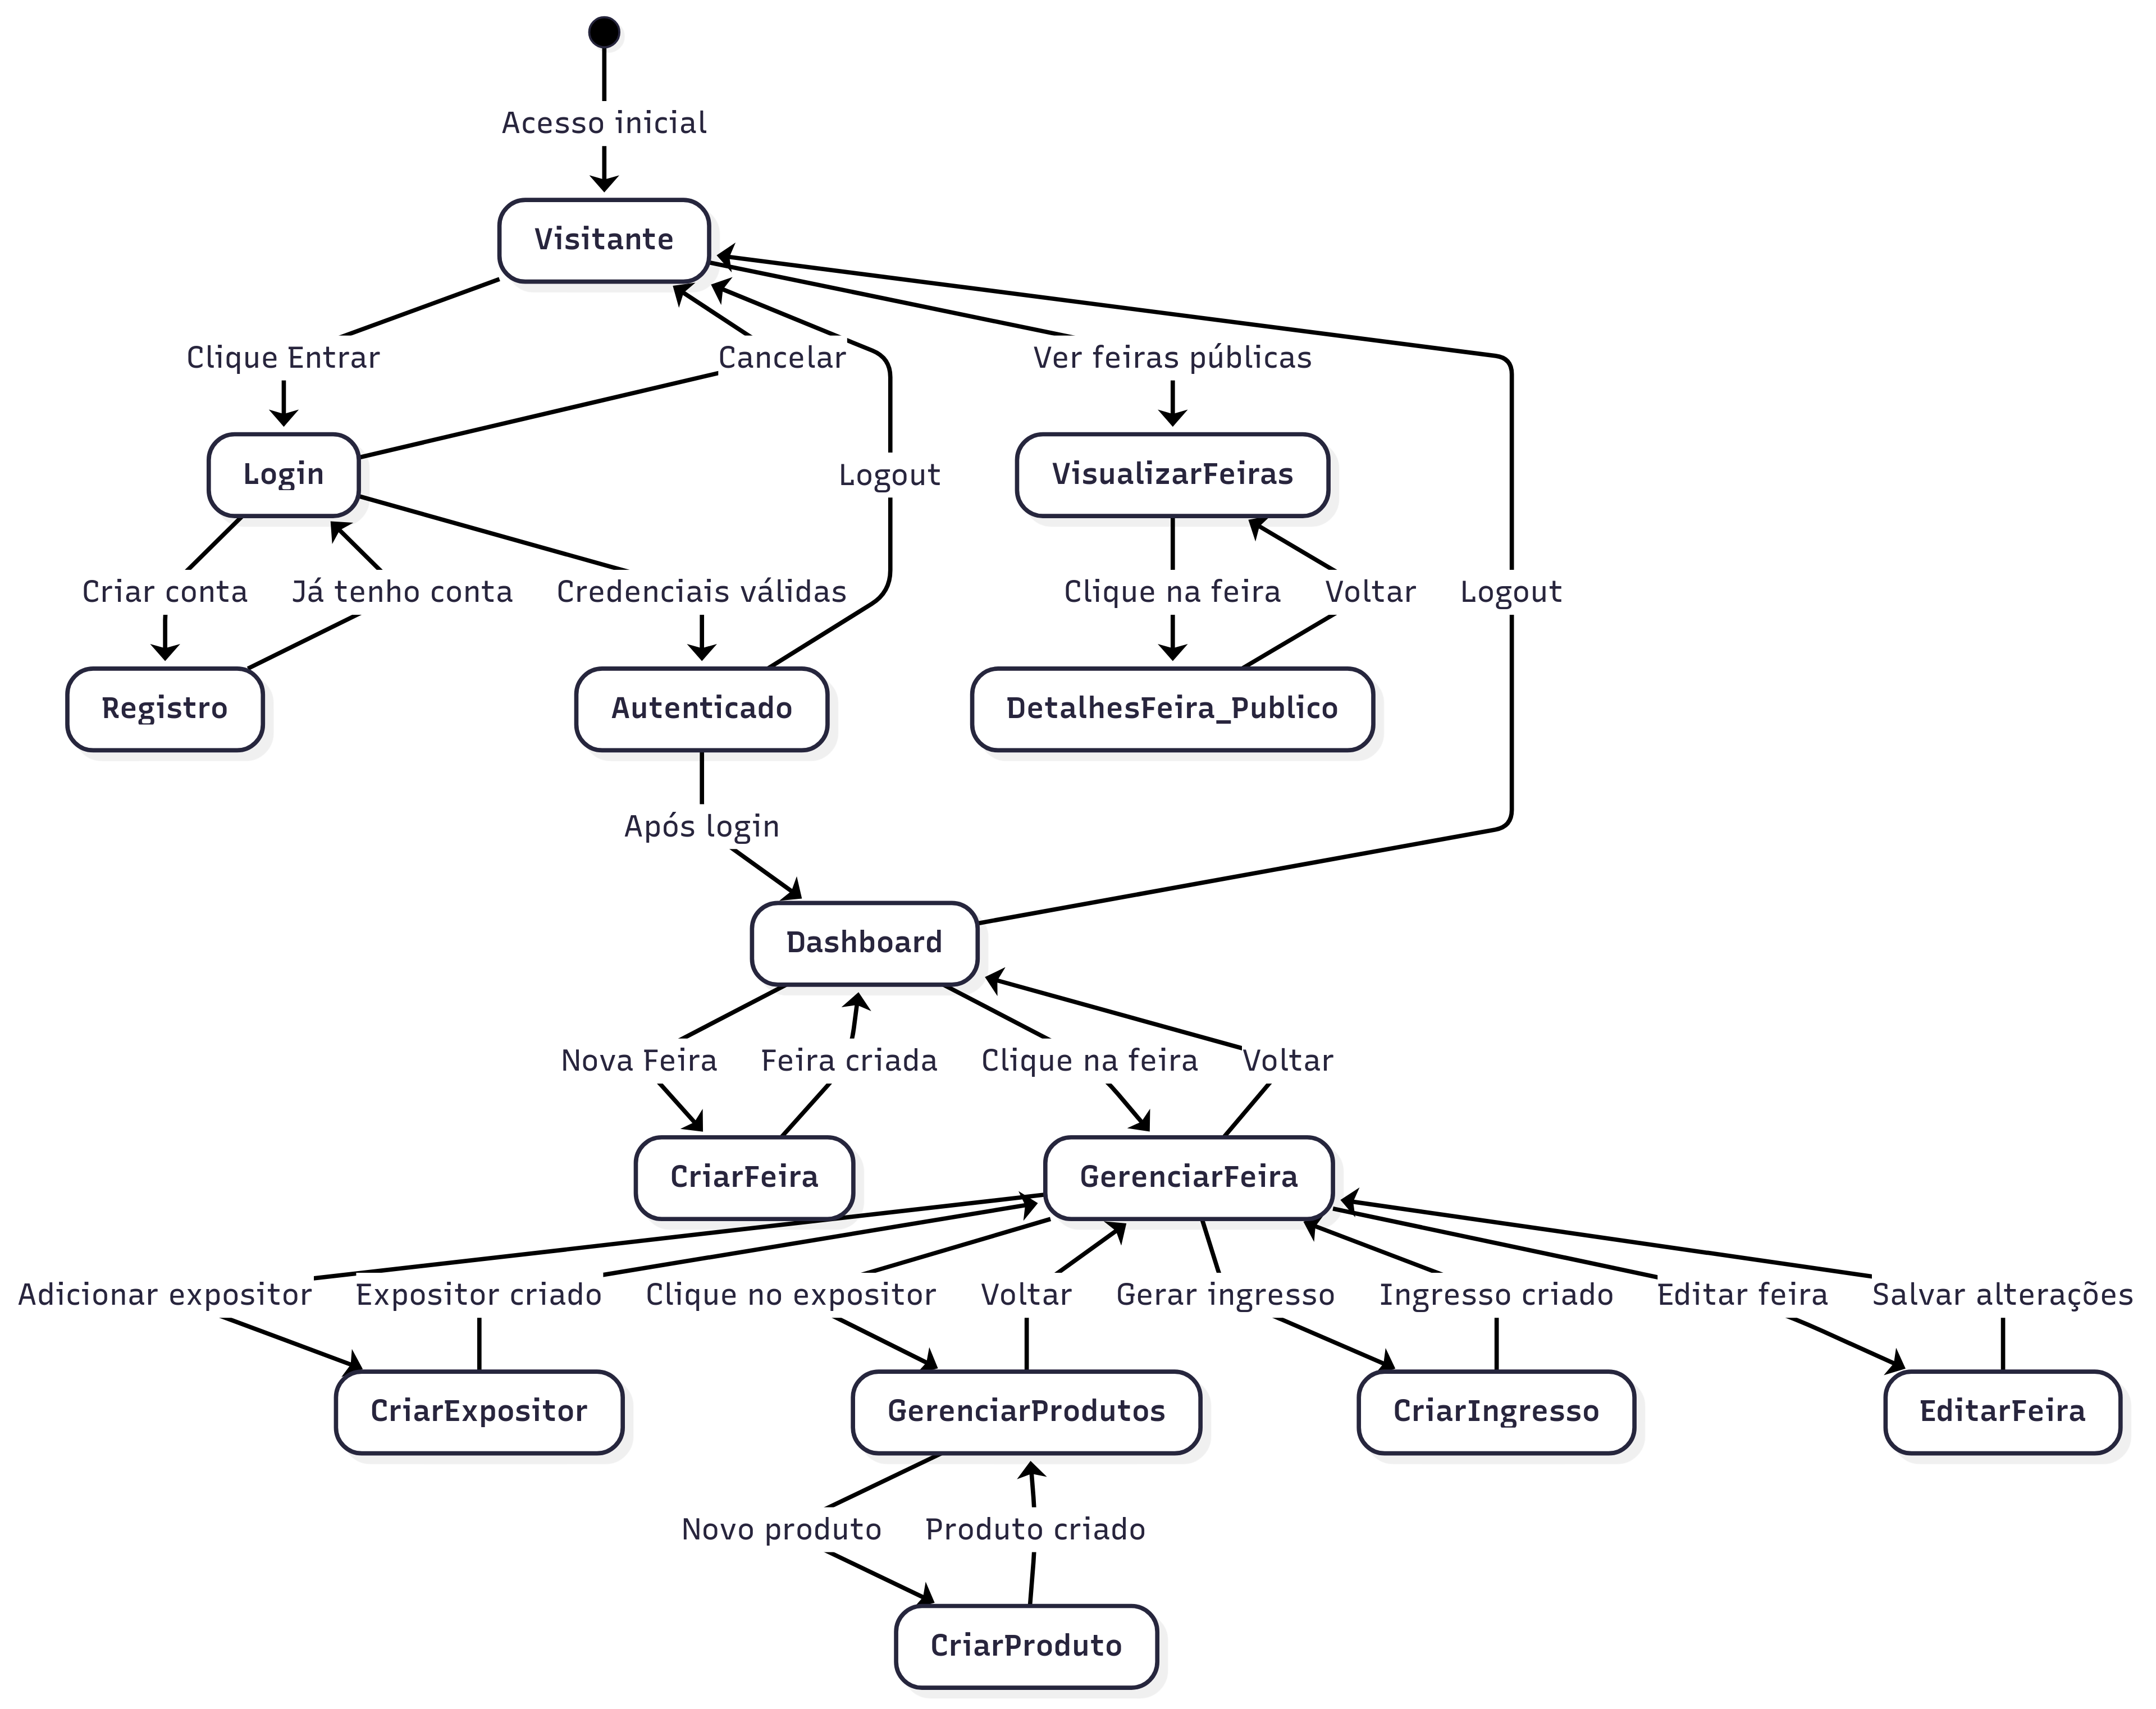
\includegraphics[width=0.9\textwidth]{diagrams/diagrama_estados_usuario.png}
\caption{Diagrama de estados e transições do usuário}
\label{fig:diagrama_estados}
\end{figure}

\textbf{Estados principais identificados:}
\begin{itemize}
    \item \textbf{Visitante}: Estado inicial, acesso público às informações
    \item \textbf{Login/Registro}: Estados de autenticação
    \item \textbf{Autenticado}: Usuário logado com acesso completo
    \item \textbf{Dashboard}: Visão geral das feiras do usuário
    \item \textbf{Gestão de Feira}: Estados de criação e edição
    \item \textbf{Gestão de Expositores}: Cadastro e manutenção
    \item \textbf{Gestão de Produtos}: Catálogo por expositor
    \item \textbf{Gestão de Ingressos}: Emissão e controle
\end{itemize}

\subsection{Fluxo de Criação de Feira}

\textbf{Processo completo:}
\begin{enumerate}
    \item Usuário clica em "Nova Feira"
    \item Preenchimento do formulário modal
    \item Validação dos campos obrigatórios
    \item Criação da feira no sistema
    \item Retorno ao dashboard com feira visível
    \item Acesso aos detalhes para gestão completa
\end{enumerate}

\section{Wireframes das Telas Principais}

Este documento apresenta o storyboard composto por wireframes das principais telas do Sistema de Gestão de Feiras (SGF). Os wireframes foram desenvolvidos como esboços funcionais e posteriormente implementados como protótipo real, sendo as imagens apresentadas capturas das telas efetivamente desenvolvidas, demonstrando a evolução do projeto desde o design até a implementação completa.

\subsection{Tela 1: Interface Inicial (Visitante)}

A tela inicial apresenta o sistema para usuários não autenticados, mostrando a mensagem de boas-vindas quando não há feiras cadastradas.

\begin{figure}[H]
\centering
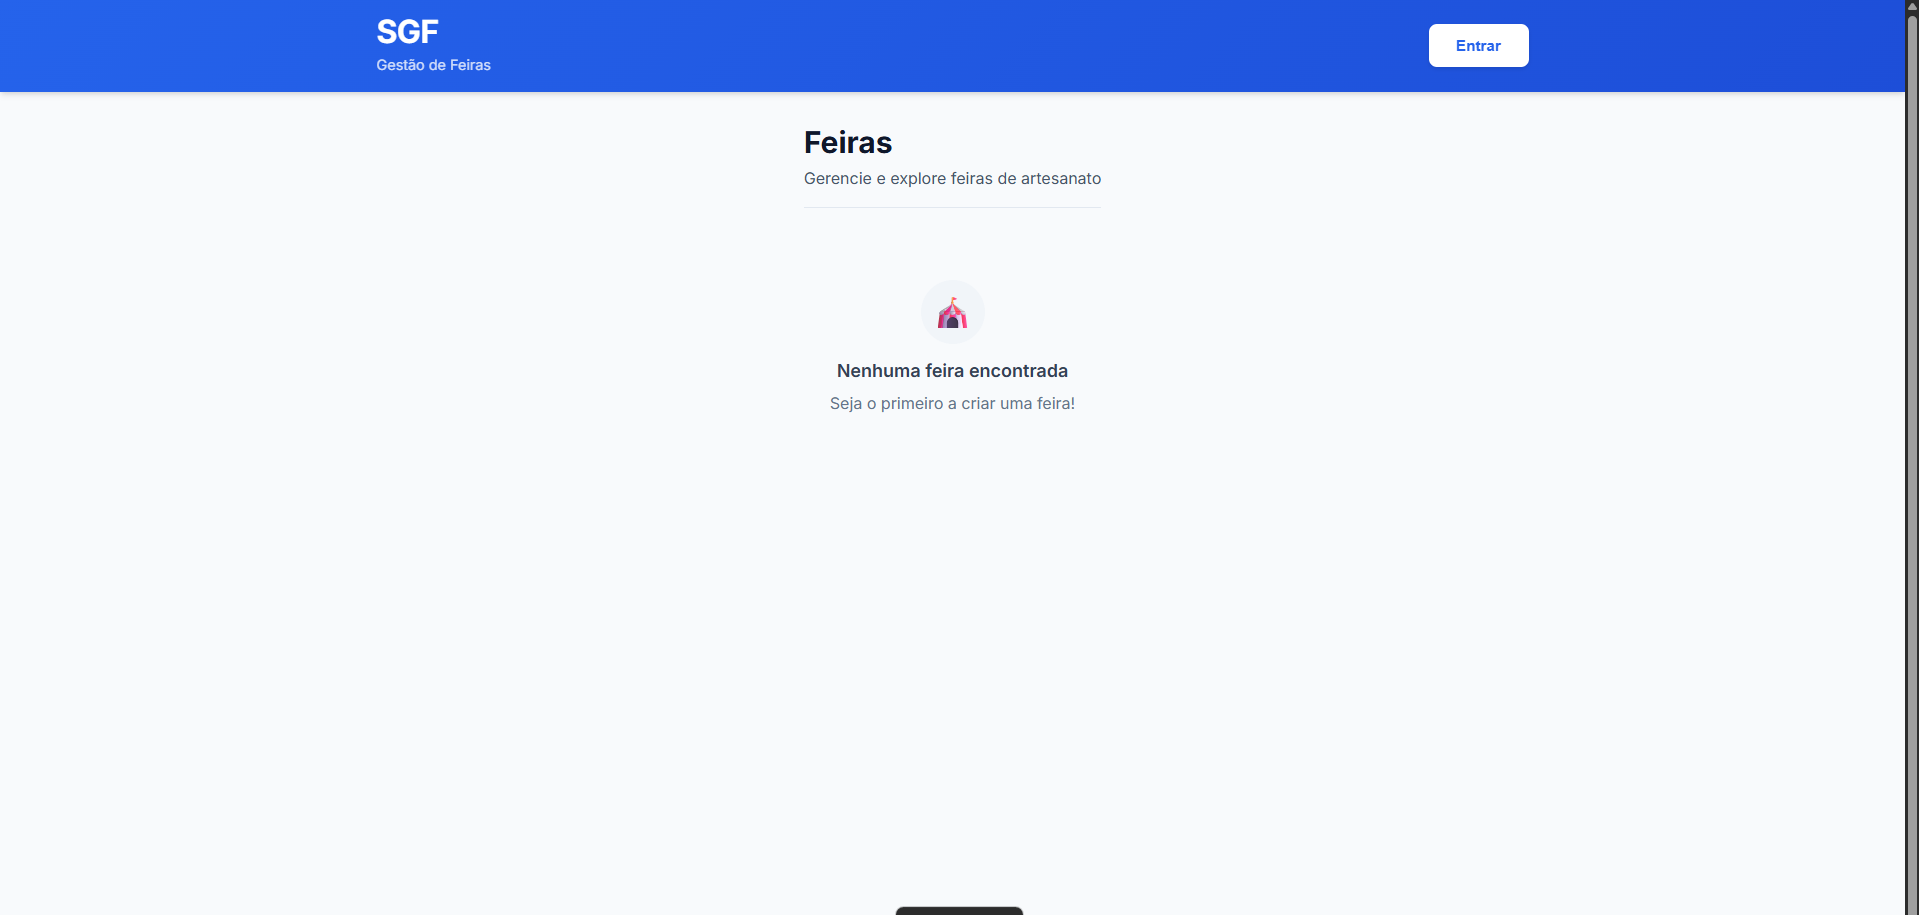
\includegraphics[width=0.9\textwidth]{wireframes/01_tela_inicial_visitante.png}
\caption{Tela inicial do sistema para visitantes}
\label{fig:tela_inicial}
\end{figure}

\textbf{Elementos principais:}
\begin{itemize}
    \item Header com logo "SGF" e botão "Entrar" posicionado à direita
    \item Título "Feiras" com subtítulo explicativo
    \item Mensagem indicando ausência de feiras cadastradas
    \item Layout limpo e responsivo
\end{itemize}

\subsection{Tela 2: Modal de Login}

Modal centralizado para autenticação de usuários com design moderno e campos de validação.

\begin{figure}[H]
\centering
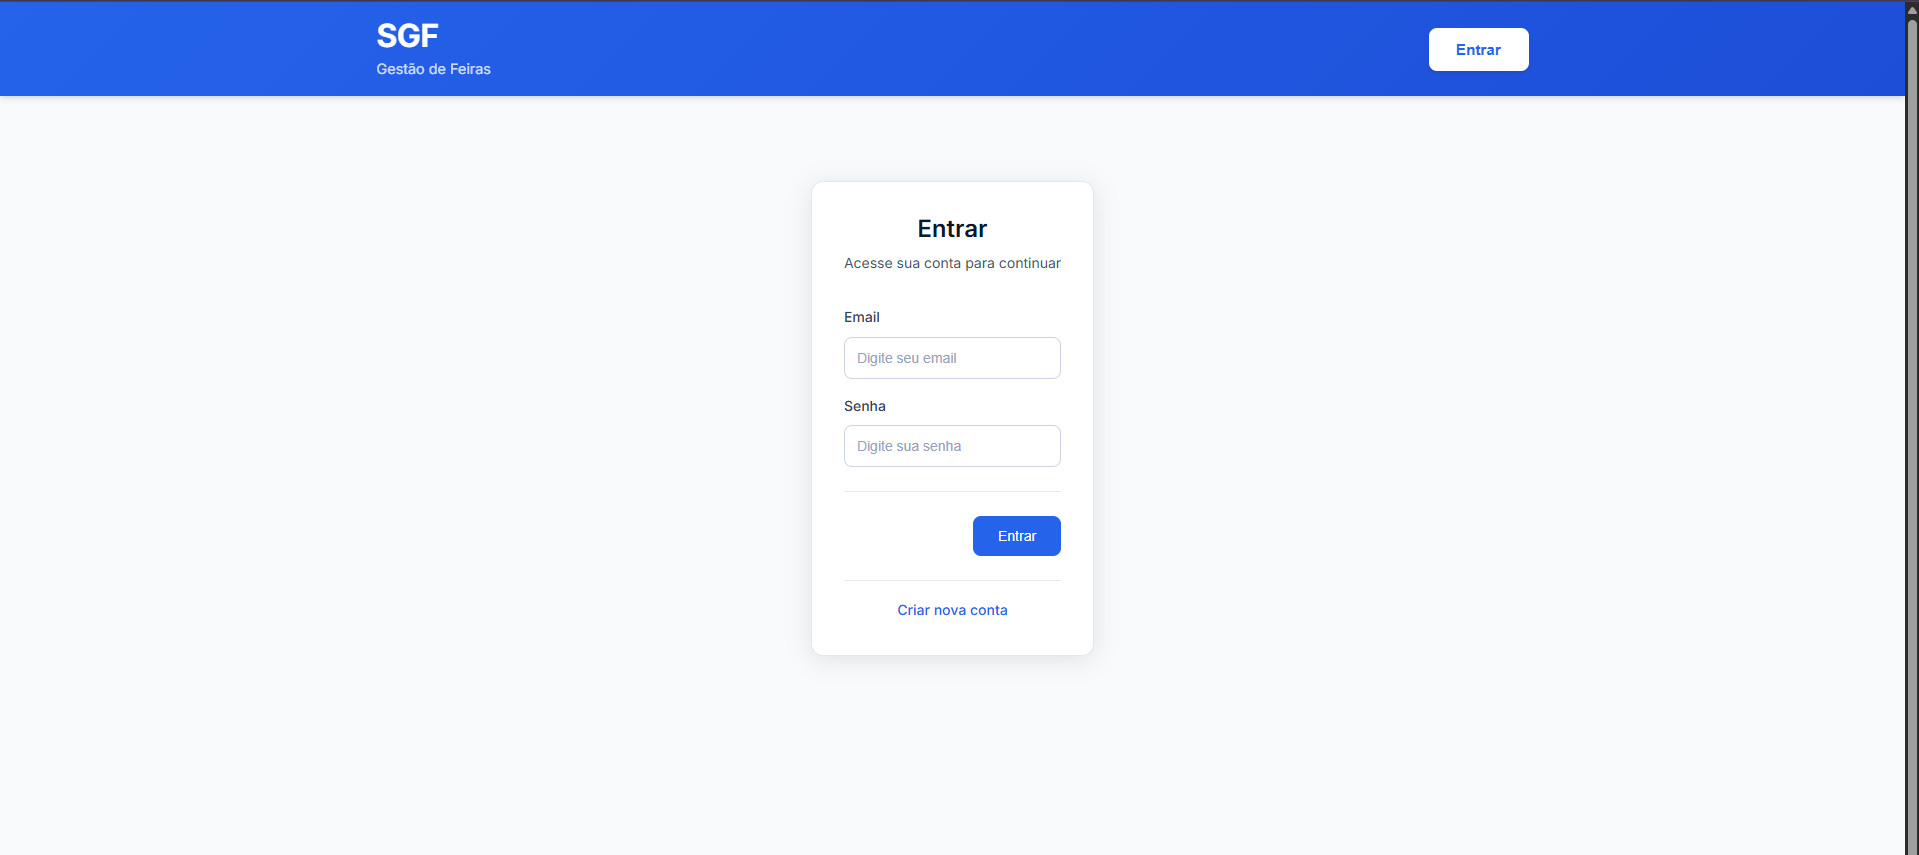
\includegraphics[width=0.7\textwidth]{wireframes/02_modal_login.png}
\caption{Modal de autenticação - Login}
\label{fig:modal_login}
\end{figure}

\textbf{Funcionalidades:}
\begin{itemize}
    \item Formulário responsivo com campos Email e Senha
    \item Botão "Entrar" destacado
    \item Link para "Criar nova conta"
    \item Overlay escuro de fundo
    \item Design de card com sombra e bordas arredondadas
\end{itemize}

\subsection{Tela 3: Modal de Registro}

Formulário de cadastro para novos usuários com campos adicionais.

\begin{figure}[H]
\centering
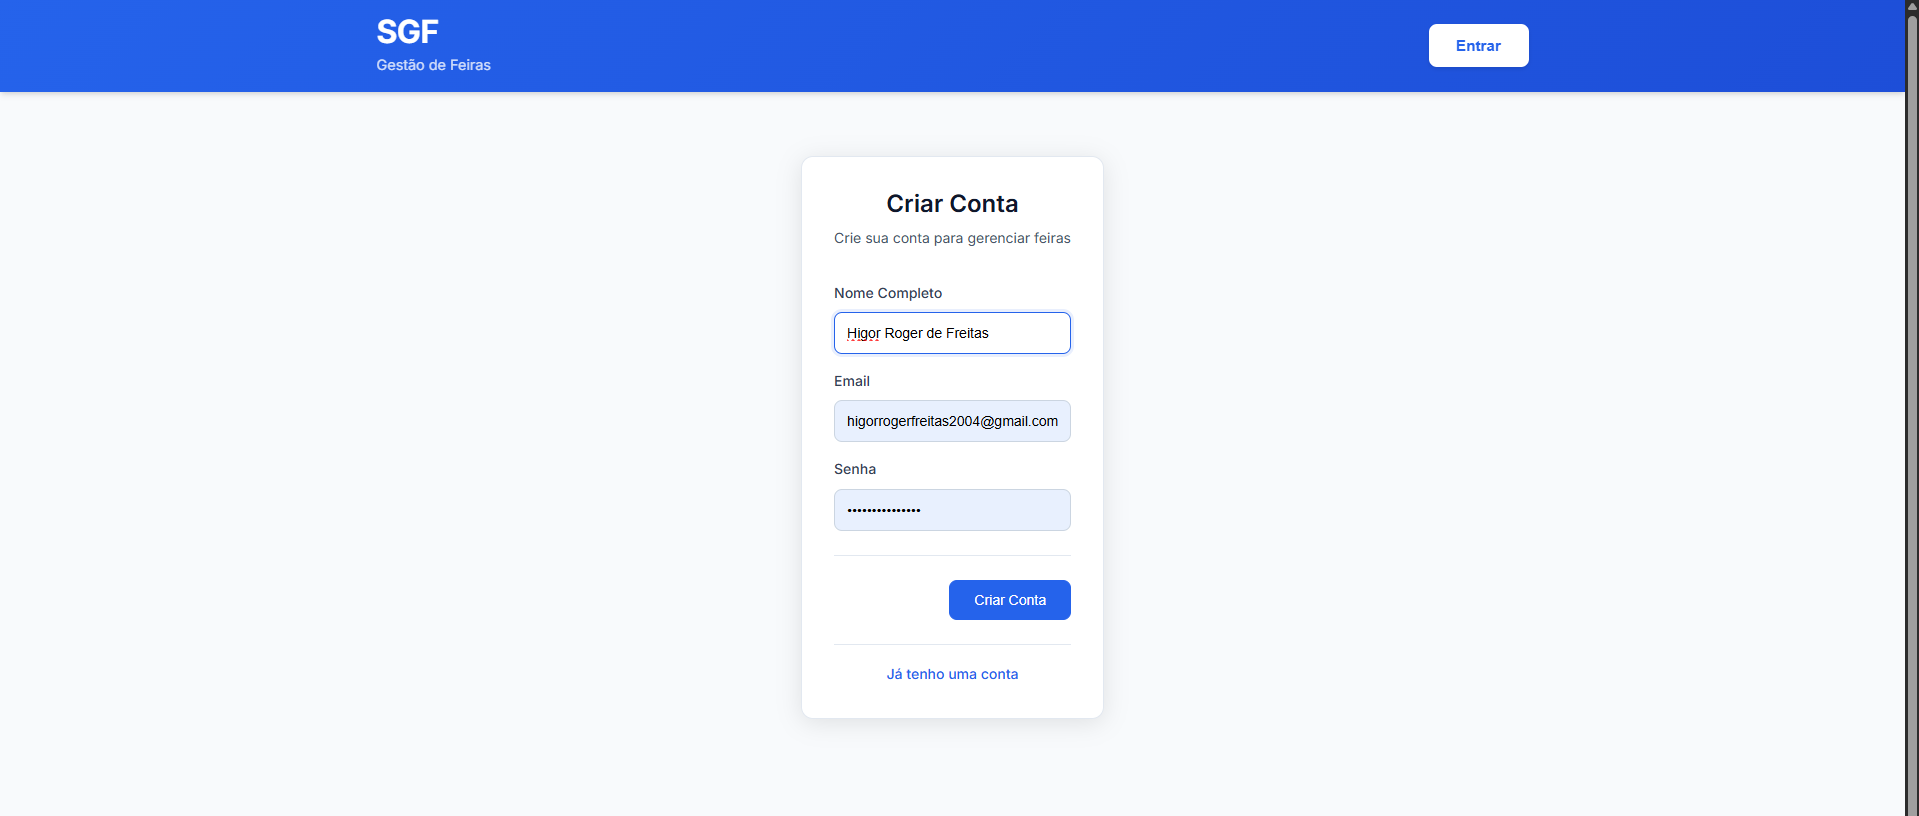
\includegraphics[width=0.7\textwidth]{wireframes/03_modal_registro.png}
\caption{Modal de autenticação - Registro}
\label{fig:modal_registro}
\end{figure}

\textbf{Componentes:}
\begin{itemize}
    \item Campo adicional "Nome Completo"
    \item Validação de email
    \item Botão "Criar Conta" em destaque
    \item Alternância com tela de login
\end{itemize}

\subsection{Tela 4: Dashboard Logado (Vazio)}

Interface inicial para usuários autenticados quando não há feiras cadastradas.

\begin{figure}[H]
\centering
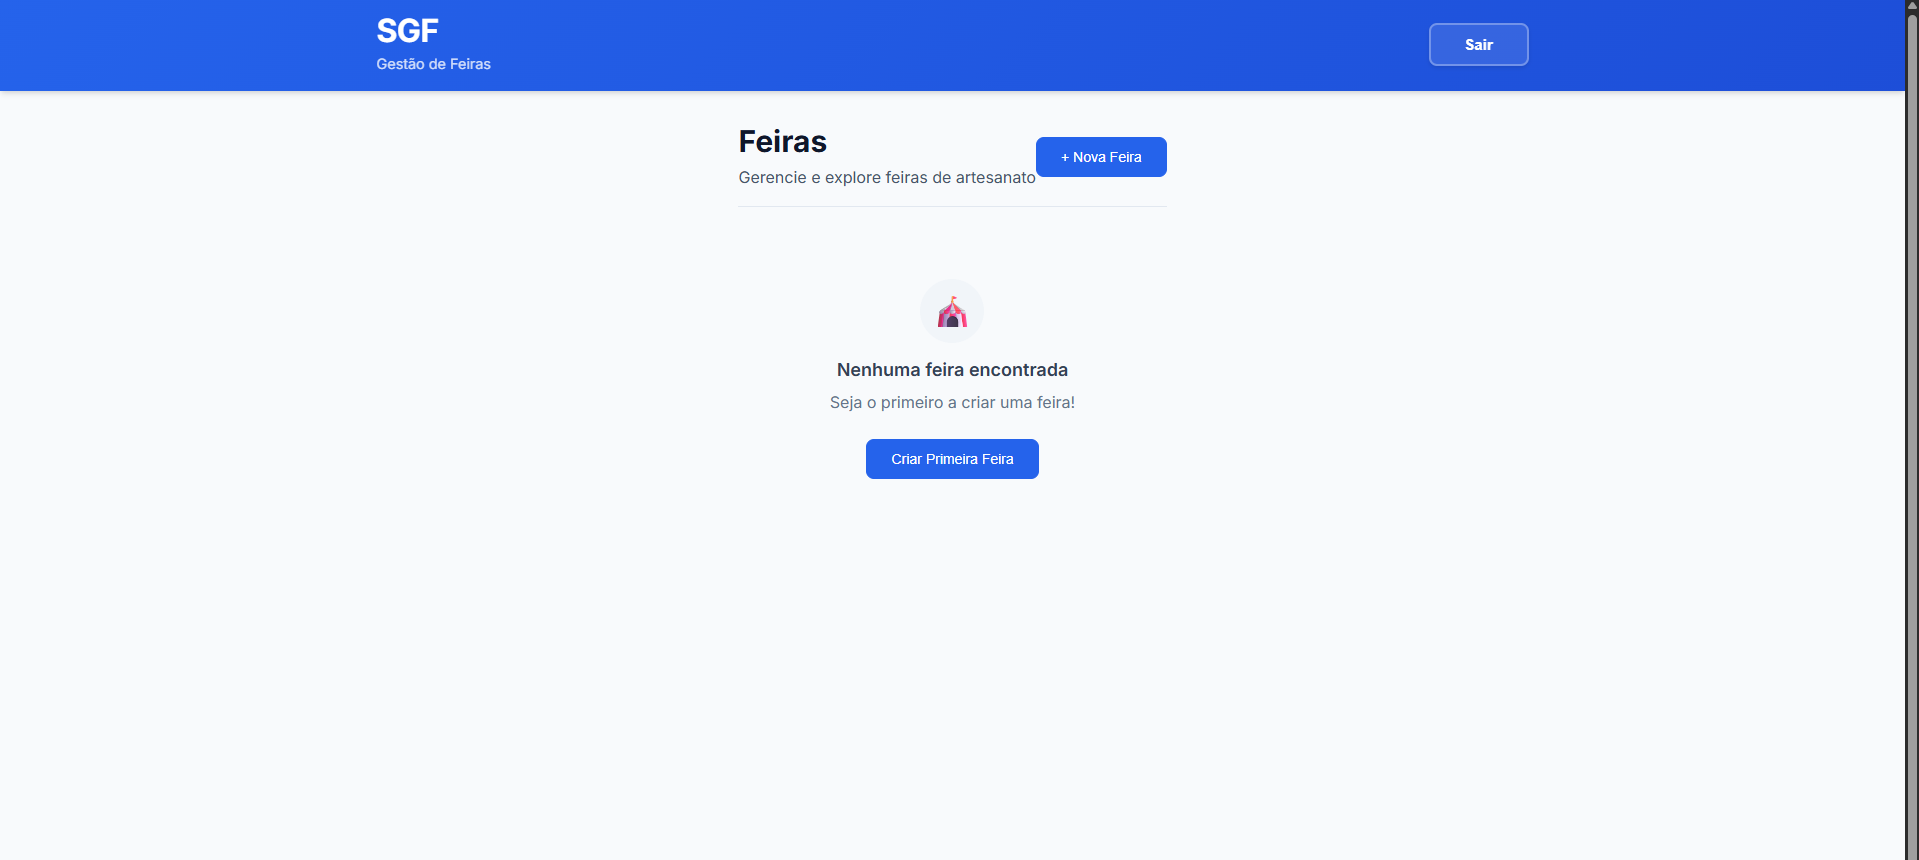
\includegraphics[width=0.9\textwidth]{wireframes/04_dashboard_logado_vazio.png}
\caption{Dashboard para usuário logado sem feiras}
\label{fig:dashboard_vazio}
\end{figure}

\textbf{Elementos para usuários autenticados:}
\begin{itemize}
    \item Header atualizado com botão "Sair"
    \item Botão "Nova Feira" em destaque
    \item Mensagem incentivando criação da primeira feira
    \item Layout preparado para exibição de conteúdo
\end{itemize}

\subsection{Tela 5: Modal de Criação de Feira}

Formulário modal completo para cadastro de novas feiras com todos os campos necessários.

\begin{figure}[H]
\centering
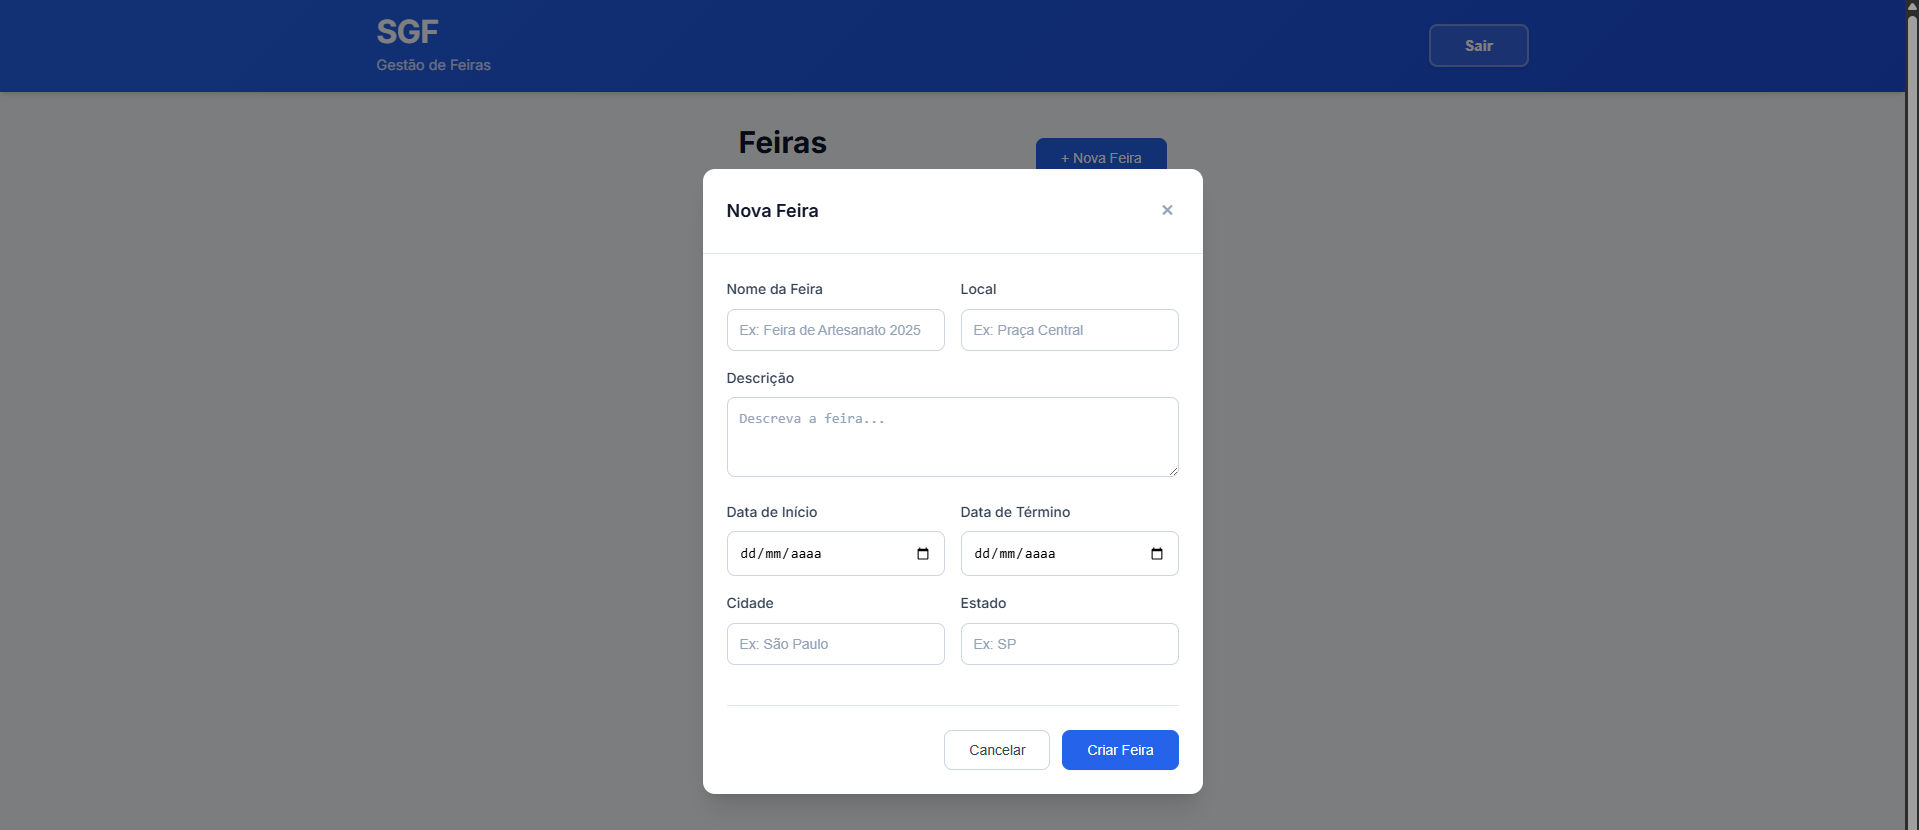
\includegraphics[width=0.8\textwidth]{wireframes/05_modal_criar_feira.png}
\caption{Formulário de criação de feira}
\label{fig:criar_feira}
\end{figure}

\textbf{Campos do formulário:}
\begin{itemize}
    \item Nome da feira e local (linha superior em duas colunas)
    \item Descrição (campo de texto expandido)
    \item Datas de início e fim (seletores de data)
    \item Cidade e estado (linha inferior em duas colunas)
    \item Botões "Cancelar" e "Criar Feira"
\end{itemize}

\subsection{Tela 6: Dashboard com Feira Criada}

Visualização do dashboard após criação de feira, mostrando o card da feira no grid responsivo.

\begin{figure}[H]
\centering
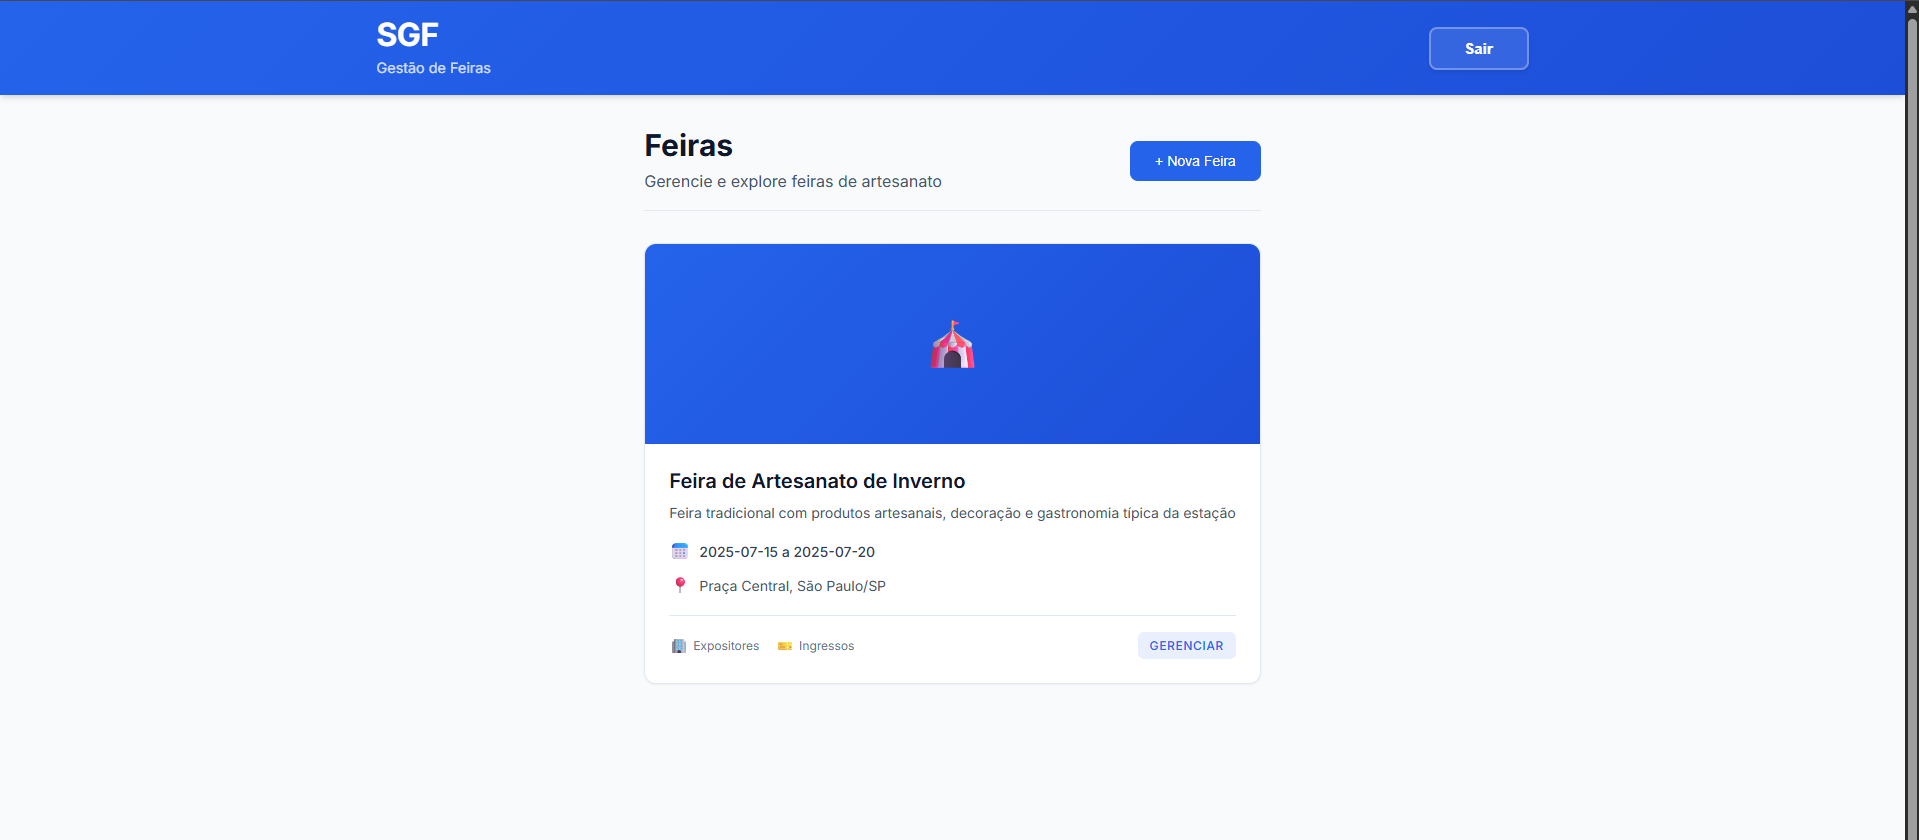
\includegraphics[width=0.9\textwidth]{wireframes/06_dashboard_com_feira.png}
\caption{Dashboard com feira cadastrada}
\label{fig:dashboard_com_feira}
\end{figure}

\textbf{Elementos do card de feira:}
\begin{itemize}
    \item Imagem de cabeçalho com ícone representativo
    \item Nome e descrição da feira
    \item Informações de data e localização com ícones
    \item Indicadores de expositores e ingressos
    \item Badge "Gerenciar" para usuários autenticados
\end{itemize}

\subsection{Tela 7: Modal de Detalhes da Feira}

Modal expandido com informações completas da feira e seções de gestão.

\begin{figure}[H]
\centering
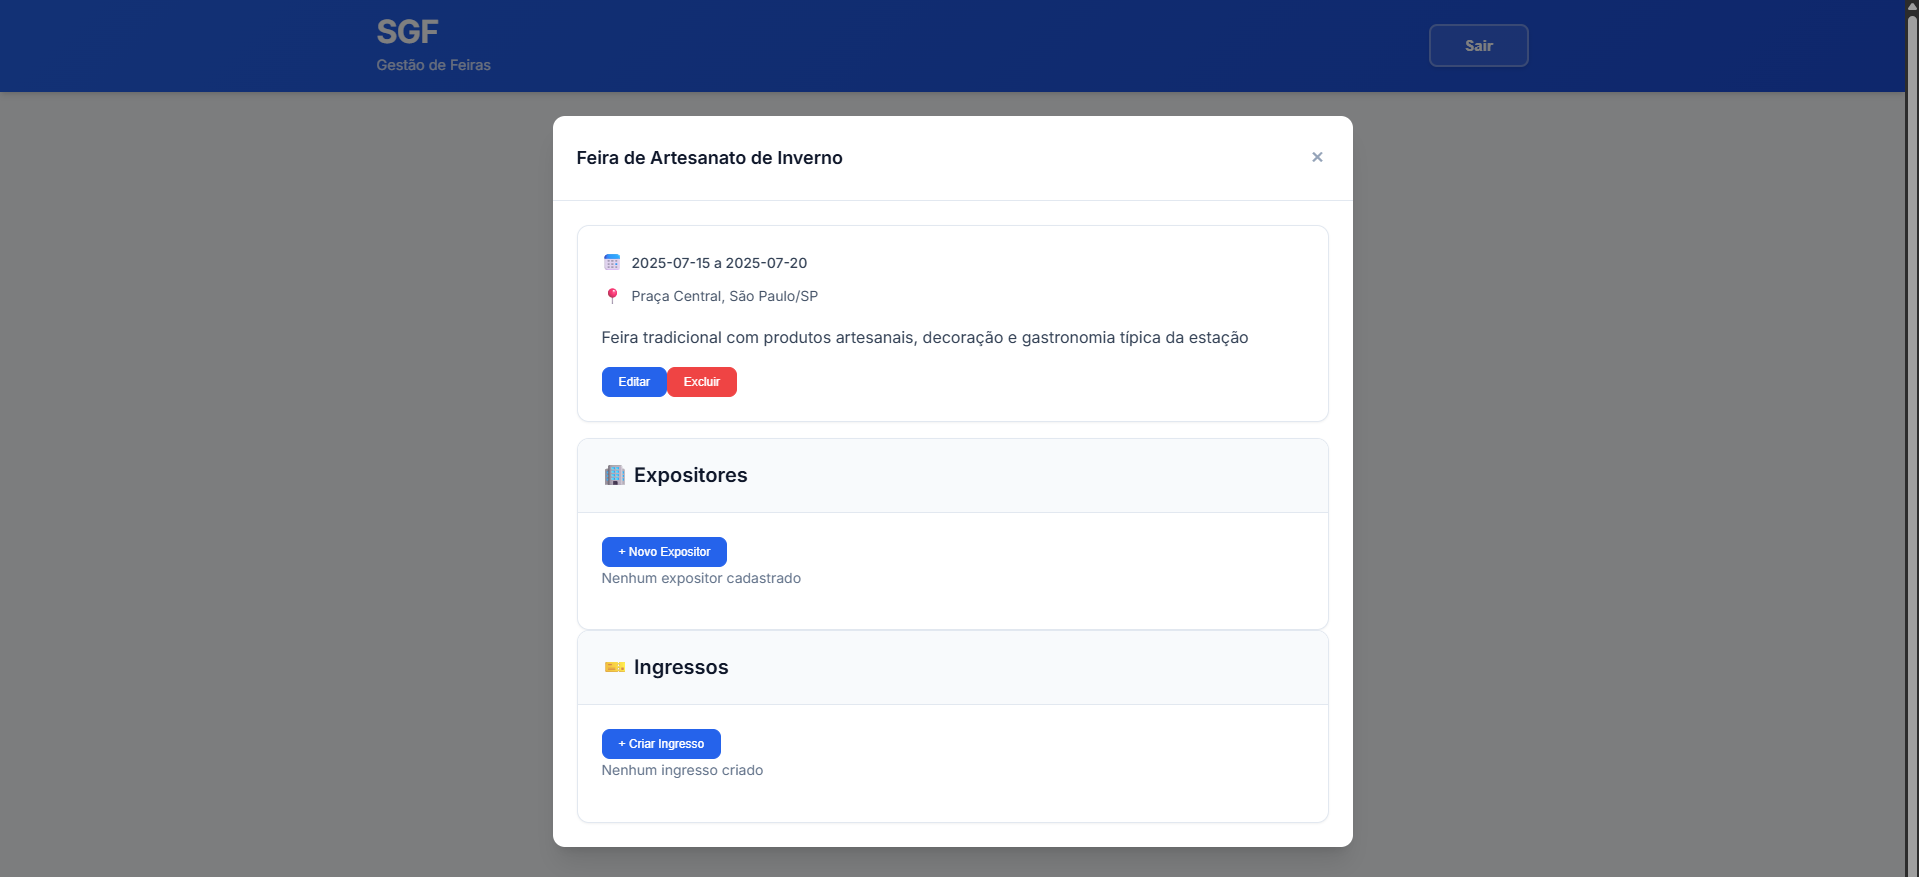
\includegraphics[width=0.9\textwidth]{wireframes/07_modal_detalhes_feira.png}
\caption{Detalhes completos da feira}
\label{fig:detalhes_feira}
\end{figure}

\textbf{Seções do modal:}
\begin{itemize}
    \item Informações principais (nome, descrição, datas, local)
    \item Botões de ação (Editar/Excluir) para o criador
    \item Seção "Expositores" com lista e botão de criação
    \item Seção "Ingressos" com gestão de tickets
    \item Layout em grid para organização das seções
\end{itemize}

\subsection{Tela 8: Gestão de Expositores}

Interface para cadastro e visualização de expositores após criação.

\begin{figure}[H]
\centering
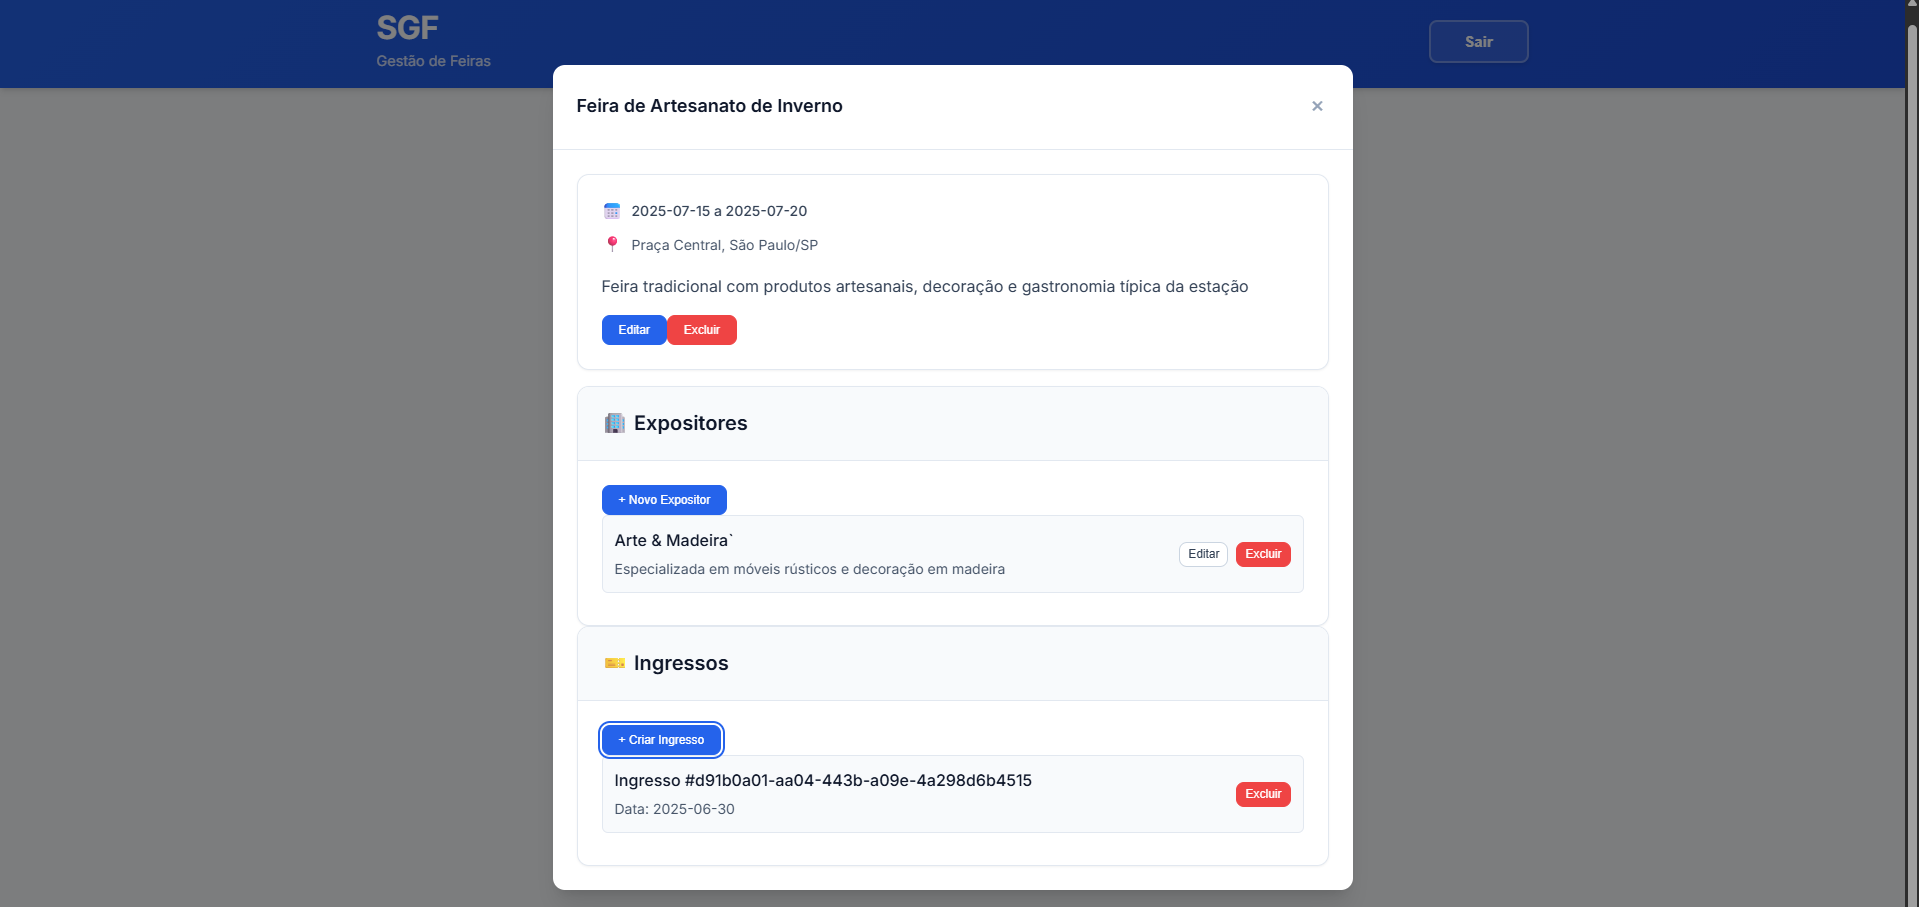
\includegraphics[width=0.9\textwidth]{wireframes/08_criar_expositor.png}
\caption{Gestão de expositores}
\label{fig:gestao_expositores}
\end{figure}

\textbf{Funcionalidades:}
\begin{itemize}
    \item Lista compacta de expositores criados
    \item Informações: nome, descrição e contato
    \item Botões de ação (Editar/Excluir) por item
    \item Interface integrada no modal de detalhes
\end{itemize}

\subsection{Tela 9: Gestão de Produtos do Expositor}

Interface para cadastro de produtos vinculados a um expositor específico.

\begin{figure}[H]
\centering
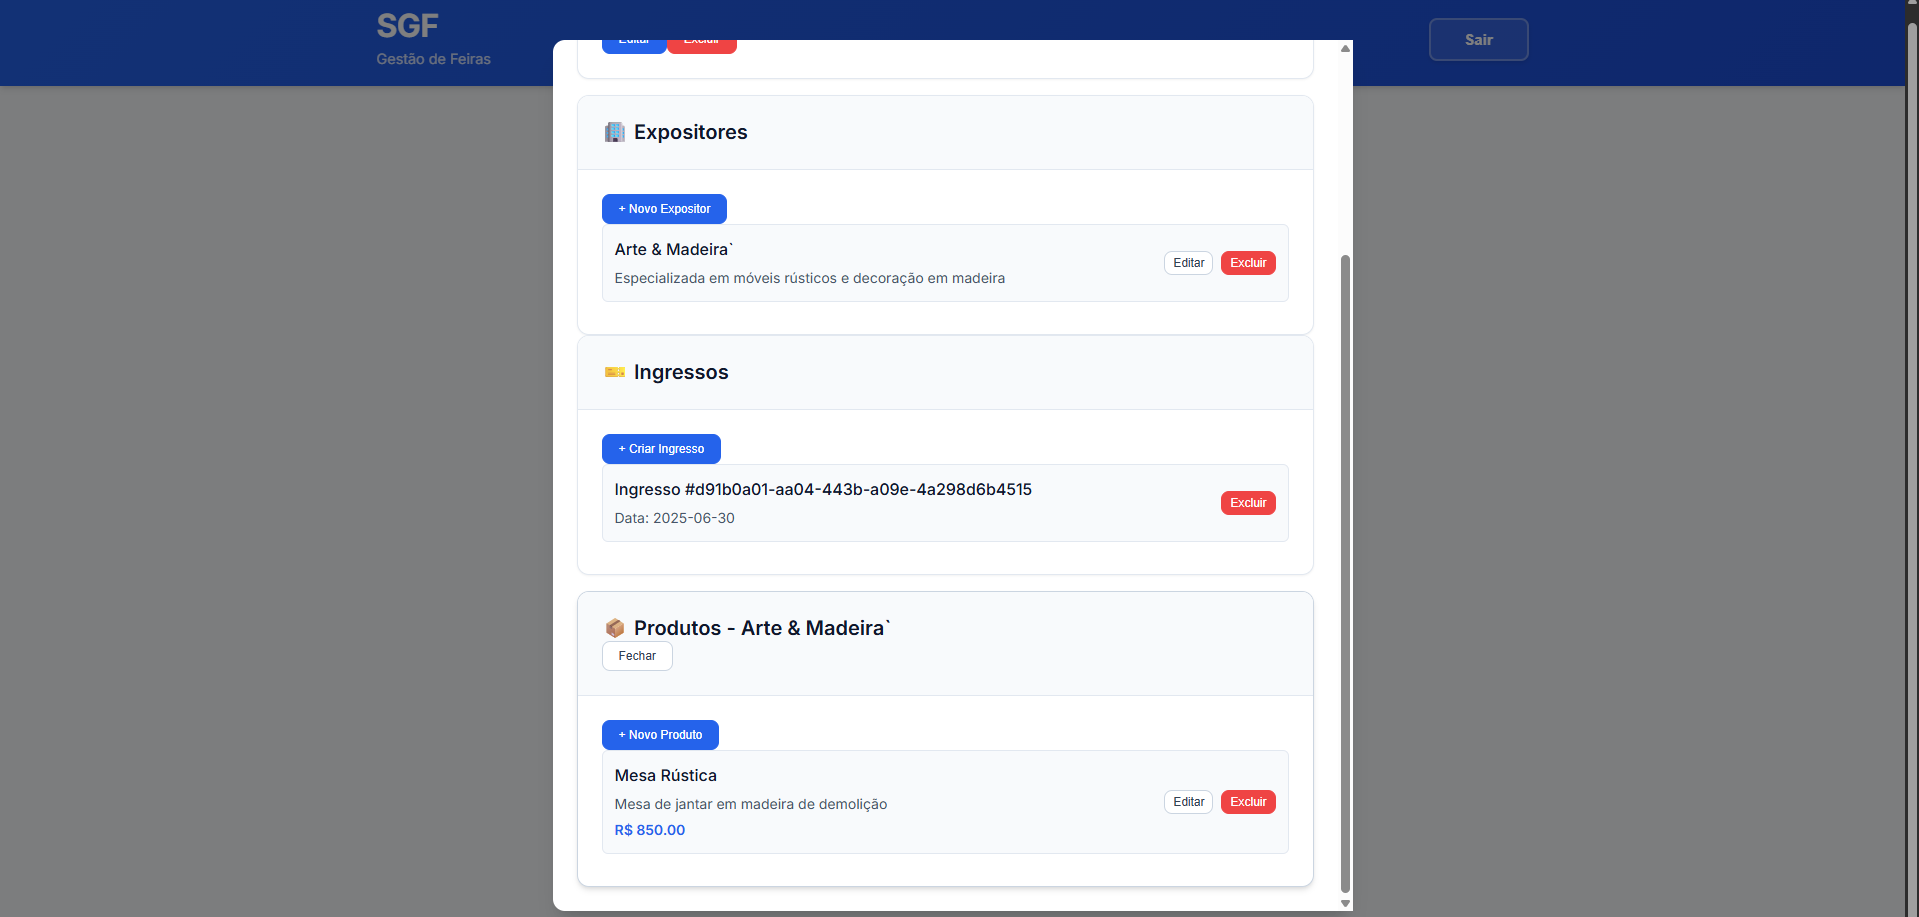
\includegraphics[width=0.9\textwidth]{wireframes/09_produtos_expositor.png}
\caption{Gestão de produtos por expositor}
\label{fig:gestao_produtos}
\end{figure}

\textbf{Elementos:}
\begin{itemize}
    \item Seção expandida mostrando produtos do expositor
    \item Informações: nome, descrição e preço formatado
    \item Botão "Novo Produto" para adição
    \item Lista organizada com ações por produto
\end{itemize}

\subsection{Tela 10: Visualização para Visitantes (Com Feira)}

Tela inicial mostrando feiras disponíveis para usuários não autenticados.

\begin{figure}[H]
\centering
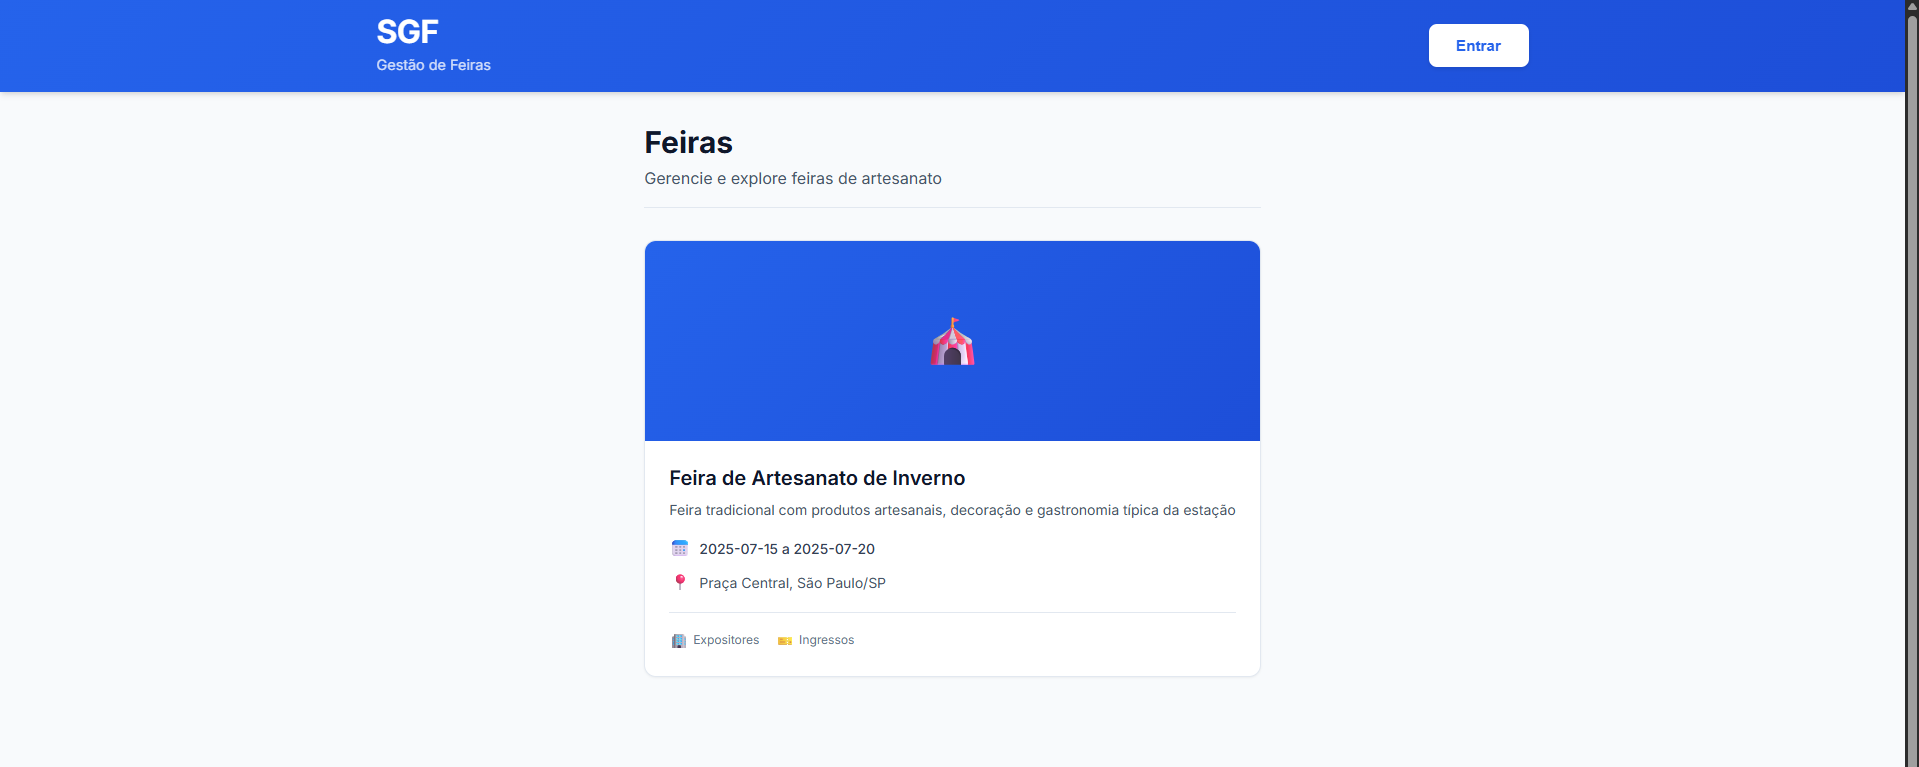
\includegraphics[width=0.9\textwidth]{wireframes/10_tela_visitante_com_feira.png}
\caption{Tela para visitantes com feiras disponíveis}
\label{fig:visitante_feiras}
\end{figure}

\textbf{Características:}
\begin{itemize}
    \item Cards de feira visíveis para visualização pública
    \item Informações completas sem opções de edição
    \item Layout idêntico ao usuário logado, mas sem ações de gestão
\end{itemize}

\subsection{Tela 11: Detalhes da Feira para Visitantes}

Modal de detalhes acessível para usuários não autenticados.

\begin{figure}[H]
\centering
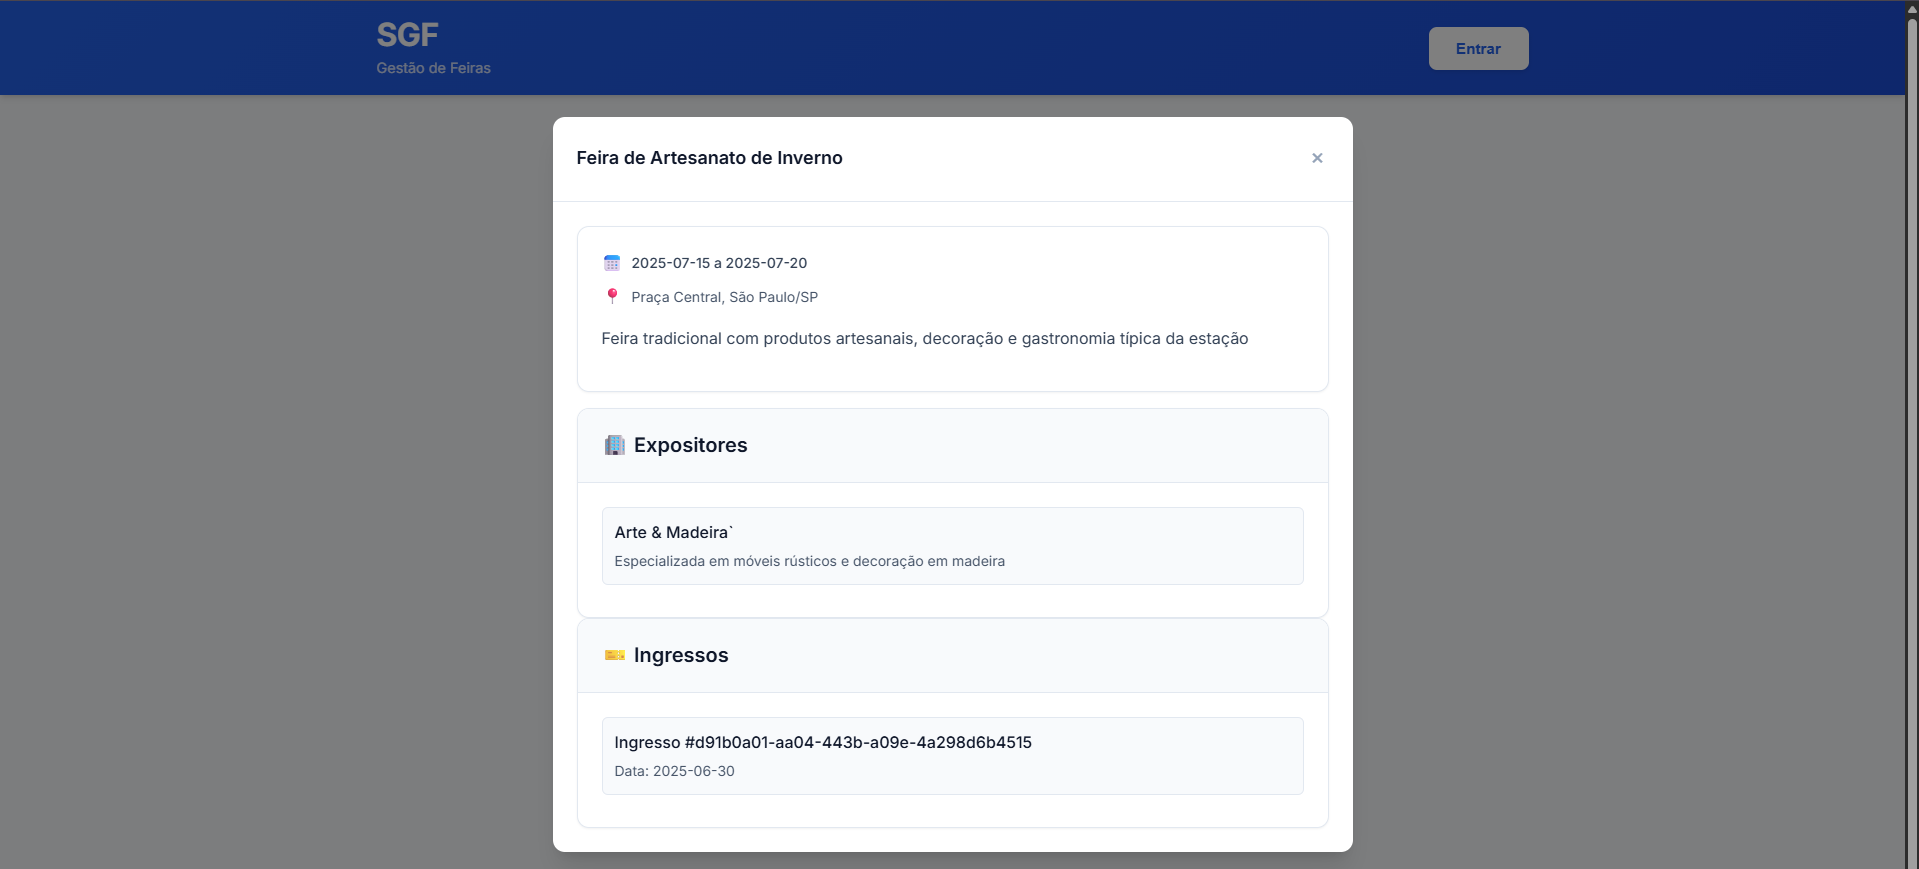
\includegraphics[width=0.9\textwidth]{wireframes/11_visitante_feira_detalhes.png}
\caption{Detalhes da feira para visitantes}
\label{fig:visitante_detalhes}
\end{figure}

\textbf{Diferenças para visitantes:}
\begin{itemize}
    \item Ausência de botões de edição/exclusão
    \item Informações de expositores e produtos visíveis
    \item Layout somente leitura
    \item Foco na visualização de informações públicas
\end{itemize}

\section{Sistema de Design}

\subsection{Paleta de Cores}

\begin{itemize}
    \item \textbf{Primary Blue:} \#2563EB (Azul principal - header e botões primários)
    \item \textbf{Primary Dark:} \#1D4ED8 (Azul escuro - hover states)
    \item \textbf{White:} \#FFFFFF (Fundo de cards e modais)
    \item \textbf{Gray 50:} \#F8FAFC (Fundo da aplicação)
    \item \textbf{Gray 600:} \#475569 (Texto secundário)
    \item \textbf{Gray 900:} \#0F172A (Texto principal)
\end{itemize}

\subsection{Tipografia}

\begin{itemize}
    \item \textbf{Fonte:} Inter (Google Fonts)
    \item \textbf{Tamanhos:} 14px (corpo), 16px (labels), 20px (títulos), 32px (logo)
    \item \textbf{Pesos:} 400 (Regular), 500 (Medium), 600 (Semibold), 700 (Bold)
\end{itemize}

\subsection{Componentes Implementados}

\begin{itemize}
    \item \textbf{Header:} Gradiente azul com logo e ações à direita
    \item \textbf{Cards:} Sombra sutil, bordas arredondadas, hover effects
    \item \textbf{Modais:} Overlay escuro, container centralizado, botão de fechar
    \item \textbf{Botões:} Estados hover, cores semânticas, tamanhos variados
    \item \textbf{Formulários:} Labels claros, validação visual, layout responsivo
\end{itemize}

\section{Responsividade}

\subsection{Implementação}
O sistema foi desenvolvido com abordagem mobile-first, garantindo funcionamento adequado em todos os dispositivos através de:

\begin{itemize}
    \item \textbf{Grid Responsivo:} Adaptação automática do número de colunas
    \item \textbf{Modais Adaptativos:} Ajuste de tamanho conforme viewport
    \item \textbf{Header Flexível:} Reorganização em telas menores
    \item \textbf{Tipografia Fluida:} Escalas adequadas para cada dispositivo
\end{itemize}

\end{document} 